\chapterimage{chapter_head_2.pdf} % Chapter heading image

\chapter{\textcolor{blue}{Fundamentos de notação musical}}
Nas seguintes sub seções abordaremos alguns conceitos de notação musical;
porem, não aprofundaremos demasiado em toda a teoria musical, 
devido a que as explicações mostradas aqui estão
orientadas para um público interessado na dança, que precisa numa primeira 
aproximação à música, conhecer rapidamente conceitos básicos. 
Mas, empoderamos a curiosidade de todos os leitores a aprofundar mais nestos temas, 
para este efeito existem na literatura muitos materiais, livros ou revistas especializadas 
\cite{medteoria}        %% Teoria Da Musica
\cite{cardoso1973curso} %% Curso Completo De Teoria Musical E Solfejo - 1o Vol.
\cite{mascarenhascurso} %% Curso Completo De Teoria Musical E Solfejo - 2o Vol.
\cite{grabner2001teoria}%% Teoría general de la música 
\cite{alves2004teoria}  %% teoria musical lições essenciais
\cite{apel1969harvard}  %% harvard diccionario
\cite{azevedocompor}    %% Como Compor Música Facilmente: métodos ou estudos para teoria, canto e solfejo (NOPDF)
\cite{adolfo2002musica}.%% Musica: Leitura, Conceitos, Exercicios (NOPDF)

%%%%%%%%%%%%%%%%%%%%%%%%%%%%%%%%%%%%%%%%%%%%%%%%%%%%%%%%%%%%%%%%%%%%%%%%%%%%%%%%
\section{Componentes da música}

A música; na sua forma mais básica,  é um conjunto de sons; esta é criada ao combinar na justa medida: 
ingênio, técnica e arte.

Entre as características de um som temos \cite[pp. 12]{medteoria} :
\begin{description}
\item [Altura:] \label{sec:pos:Altura} 
Também chamado \textbf{tom}\footnote{A palavra tom tem vários significados em música, 
outro significado pode ser um intervalo ou distancia em frequência, 
utilizado na escala diatônica, para mais detalhes ir a Seção \ref{sec:notasmusicais}}, representa a frequência de vibração (principal) da onda mecânica que gera o sonido.
Isto é, que terão um altura maior os sonidos com maior frequência de vibração mecânica (mais agudos), 
e uma altura menor sonidos mais graves.
\begin{example}
A campainha pra chamar ao atendente de um hotel tem uma altura maior,
que a campana da igreja, que é tocada ao médio dia, que tem um sonido mais grave.
\end{example} 
\index{Altura}\index{Tom}
\item [Duração:] \label{sec:pos:Duracion}
Representa a longitude temporal, durante o qual um sonido será executado.
\begin{example}
Podemos assoviar durante um tempo, curto, longo, muito longo, etc.
\end{example} 
\index{Duração}
\item [Intensidade:] \label{sec:pos:Intensidade}
Se refere ao volume sonoro ou à potencia do sonido executado, 
de modo que o som pode ter intensidades, por exemplo: fracas, fortes, muito fortes, etc.  
\begin{example}
Si escolhemos dois pedaços de madeira e batimos eles um contra outro, 
podemos gerar sons com diferente intensidade, dependendo da força com que realizemos os batimentos.
\end{example} 
\index{Intensidade}
\item [Timbre:] \label{sec:pos:timbre}
Na definição da altura de um som, referenciamos esta seguindo a sua frequência principal,
porem um som não está composto exclusivamente por vibrações a esta frequência.
Na pratica os sons contem muitas outras frequências de vibração, acontecendo simultaneamente e 
que se manifestam com menor intensidade.
A combinação de todas estas frequências de vibração é o que gera o som que escutamos;
assim, a essa especifica configuração de frequências a chamamos como o timbre ou
a ``\textbf{cor}'' do som.
\begin{example}
Se geramos dois sonidos com a mesma altura; mas, um sonido executado por uma flauta,
e o outro por um violão, ambos sonidos terão diferentes timbres ou cores.
\end{example} 
\index{Timbre}
\end{description}
~\\

Conhecidas estas definições básicas, e procurando estruturas mais complexas na música,
podemos distinguir alguns componentes com que esta é constituída, 
por exemplo temos:

\begin{description}
\item [Ritmo:] \label{sec:pos:Ritmo}
Se refere a distribuição temporal da execução dos sonidos e a proporção na duração destes. 
Asim, o ritmo carateriza a música no âmbito temporal \cite[pp. 11]{medteoria}.
\index{Ritmo}
\begin{example}
Batendo palmas, criamos a sequencia de sonidos: palmas, pausa curta, palmas, palmas, pausa loga e palmas.
\end{example} 
\item [Melodia:] \label{sec:pos:Melodia}
É um conjunto de sons, que podem ter diferentes \hyperref[sec:pos:Altura]{\textbf{alturas}}, 
e que estão dispostos sequencialmente. 
A melodia representa um elemento horizontal\footnote{\label{eixohor}Eixo com múltiplas distribuições de tempo dos sons na música} na musica, 
e esta é indivisível do ritmo \cite[pp. 517]{apel1969harvard} \cite[pp. 11]{medteoria}.
\begin{example}
Se assoviamos ``parabéns pra você'', estamos executando uma melodia 
(executando diferentes sons numa distribuição temporal especifica).
\end{example} 
\index{Melodia} 
\item [Harmonia:] \label{sec:pos:Harmonia}
Conjunto de sons dispostos simultaneamente em \hyperref[sec:pos:Altura]{\textbf{alturas}} diferentes.
A harmonia representa um elemento vertical\footnote{\label{eixover}Eixo com múltiplas distribuições de frequência dos sons na música} na música \cite[pp. 371]{apel1969harvard} \cite[pp. 8]{cardoso1973curso} \cite[pp. 11]{medteoria}. 
\begin{example}
Se num piano pressionamos simultaneamente as teclas: Do, Mi e Sol. Estamos executando uma harmonia.
\end{example} 
\index{Harmonia} 
\item [Contraponto:] \label{sec:pos:Contraponto}
O termo deriva de ``punctus contra punctum'' que significa ``nota contra nota'', 
e por extensão ``melodia contra melodia''. 
Assim, falar de contraponto é equivalente a dizer, dois ou mais melodias executadas simultaneamente  
(concepção horizontal\footref{eixohor} e vertical\footref{eixover} da música)  \cite[pp. 208]{apel1969harvard} \cite[pp. 11]{medteoria}.
\begin{example}
Uma orquestra com vários músicos tocando cada um uma melodia.
\end{example} 
\index{Contraponto}
\end{description}


%%%%%%%%%%%%%%%%%%%%%%%%%%%%%%%%%%%%%%%%%%%%%%%%%%%%%%%%%%%%%%%%%%%%%%%%%%%%%%%%
\section{Figuras musicais e pausas}\index{Figuras musicais}
As figuras musicais são um conjunto de sinais (desenhos), criadas pra indicar a relação 
entre as \hyperref[sec:pos:Duracion]{\textbf{durações}} dos sons \cite[pp. 20]{medteoria}.
Assim, podemos ver na coluna dois da Tabela \ref{tab:abc-noteslengthbasic}
 um conjunto de 6 destas figuras musicais; 
a primeira coluna representa a longitude temporal (\hyperref[sec:pos:Duracion]{\textbf{duração}}) de cada uma destas figuras;
porem, todos estas durações são relativas ao valor temporal $S$, em segundos, de uma figura \Ganz.
A terceira coluna da tabela contem os nomes de cada uma destas figuras musicais. 
\begin{table}[h]
\centering
\begin{tabular}{|c||c|c||c|c|}
\hline
Duração & Figura & Nome de figura & Pausa & Nome de pausa\\ \hline
\hline
$S$    & \Ganz   & Semibreve    & \GaPa  & Pausa de Semibreve \\ \hline
$S/2$  & \Halb   & Mínima       & \HaPa  & Pausa de Mínima \\ \hline
$S/4$  & \Vier   & Semínima     & \ViPa  & Pausa de Semínima \\ \hline
$S/8$  & \Acht   & Colcheia     & \AcPa  & Pausa de Colcheia \\ \hline
$S/16$ & \Sech   & Semicolcheia & \SePa  & Pausa de Semicolcheia \\ \hline
$S/32$ & \Zwdr   & Fusa         & \ZwPa  & Pausa de fusa  \\ \hline  
\end{tabular}
\caption{Duração e símbolos de algumas figuras musicais}
\label{tab:abc-noteslengthbasic}
\end{table}


\begin{example}
Se decidimos criar uma sequencia rítmica assoviando um único tom, porem
distribuindo os tempos de duração como: Longo, curto, curto; 
repetindo esta sequencia quatro vesses. 
Poderíamos escrever esta usando figuras musicais numa representação como a mostrada na Figura \ref{fig:abc-figurasexample1}.
É importante ressaltar que assumimos que  um sonido longo dura no tempo exatamente o dobro que um curto, 
e que decidimos\footnote{É escolhida uma semínima porem pode ter sido escolhida 
qualquer outra figura, dado que o valor $S$ não está definido.}
representar um sonido de longa duração como uma semínima.

Para entender melhor a representação com figuras musicais, 
podemos ir a uma representação alternativa com um gráfico da potencia do sonido na execução dos sons,
como é representado na Figura \ref{fig:abc-figurasexample1}.
É fácil perceber como a potencia do som se mantêm, ate justo antes de iniciar 
o seguinte sonido, de modo que não existem silêncios na sequencia rítmica.
\end{example} 




\begin{figure}[h]
    \centering
    \begin{subfigure}[b]{0.9\textwidth}
 \begin{abc}[name=abc-figurasexample1]
% abcm2ps figurasexample1.abc  -O figurasexample1.ps
% ps2epsi figurasexample1.ps figurasexample1.eps
%
X: 1 % start of header
K: none stafflines=0 %K: C %% Escala de C mayor %
M:  none % M: 2/4
%T: Contratempo num compasso binário
V:1 clef=none stem=up %name="Ritmo 1"   sname="Ritmo 1"
%
[V:1] | B2 B1 B1 B2 B1 B1 B2 B1 B1 B2  B1 B1   |
%       
\end{abc}
	\caption{Sequencia rítmica usando semínimas e colcheias.}
	\label{fig:abc-figurasexample1}
    \end{subfigure}
    ~%add desired spacing between images, e. g. ~, \quad, \qquad, \hfill etc. 
      %(or a blank line to force the subfigure onto a new line)
    \begin{subfigure}[b]{0.9\textwidth}
        
\includegraphics[width=\textwidth]{chapters/cap-musica-basica/forma-figurasexample1.eps}
        \caption{Sequencia rítmica usando um gráfico indicando a potencia do sonido.}
        \label{fig:forma-figurasexample1}
    \end{subfigure}
    \caption{Sequencia rítmica.}\label{fig:total-figurasexample1}
\end{figure}


Por outro lado, assim como a duração do tempo de execução de cada som precisa uma grafia,
os silêncios ou pausas, também precisam ser indicados. 
De modo que, para cada figura musical existe uma grafia que indica um silencio da mesma duração temporal,
como pode ser visto na quarta coluna da Tabela \ref{tab:abc-noteslengthbasic}.
O nome de cada uma destas pausas está descrito na quinta coluna da mesma tabela.

\begin{example}
Similarmente ao exemplo anterior, se decidimos criar uma sequencia rítmica assoviando um único tom, porem
intercalando sons e silêncios, podemos criar um padrão rítmico como na Figura \ref{fig:total-figurasexample2}.

Podemos entender melhor a representação com figuras musicais, 
usando a representação com um gráfico da potencia do sonido na execução dos sons,
como é representado na Figura \ref{fig:forma-figurasexample2}.
Nela percebemos como a potencia do som se mantêm durante a longitude de tempo estipulada pela figura musical, 
ate justo antes de iniciar o silencio, indicado por uma linha reta.
\end{example} 

\begin{figure}[h]
    \centering
    \begin{subfigure}[b]{0.9\textwidth}
 \begin{abc}[name=abc-figurasexample2]
% abcm2ps figurasexample2.abc  -O figurasexample2.ps
% ps2epsi figurasexample2.ps figurasexample2.eps
%
X: 1 % start of header
K: none stafflines=0 %K: C %% Escala de C mayor %
M:  none % M: 2/4
%T: Contratempo num compasso binário
V:1 clef=none stem=up %name="Ritmo 1"   sname="Ritmo 1"
%
[V:1] | z1 B1 z1 B1 z2 B1 z1 B1 z1 B1 z2 B1  z1 B1   |
%       
\end{abc}
	\caption{Sequencia rítmica usando  colcheias e silencios.}
	\label{fig:abc-figurasexample2}
    \end{subfigure}
    ~%add desired spacing between images, e. g. ~, \quad, \qquad, \hfill etc. 
      %(or a blank line to force the subfigure onto a new line)
    \begin{subfigure}[b]{0.9\textwidth}
        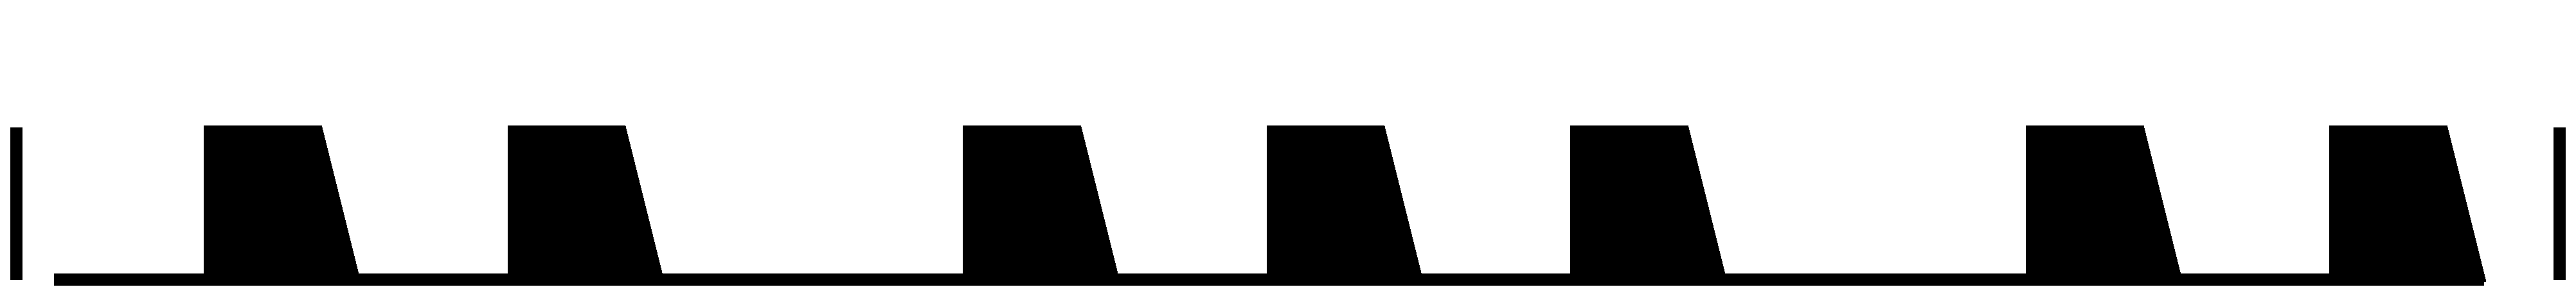
\includegraphics[width=\textwidth]{chapters/cap-musica-basica/forma-figurasexample2.eps}
        \caption{Sequencia rítmica usando um gráfico indicando a potencia do sonido.}
        \label{fig:forma-figurasexample2}
    \end{subfigure}
    \caption{Sequencia rítmica.}\label{fig:total-figurasexample2}
\end{figure}


Ate agora todos os exemplos foram sequencias rítmicas, 
pois não exploramos a possibilidade de variar a altura dos sonidos;
para poder explorar esta possibilidade devemos ter claro o conceito de pauta,
para que cada figura musical, 
além de nos proporcionar uma informação da \hyperref[sec:pos:Duracion]{\textbf{duração}}  dos sons, 
também nos de informação da \hyperref[sec:pos:Altura]{\textbf{altura}}  destes. 
Tendo estes dois fatores, altura e duração, podemos criar \hyperref[sec:pos:Melodia]{\textbf{melodias}}.

\begin{remark}
O mistério de como distinguir a pausa de mínima (\HaPa) e a pausa de semibreve (\GaPa),
será esclarecido quando desenhemos estes na \hyperref[sec:pauta]{\textbf{pauta}}.
\end{remark}

%%%%%%%%%%%%%%%%%%%%%%%%%%%%%%%%%%%%%%%%%%%%%%%%%%%%%%%%%%%%%%%%%%%%%%%%%%%%%%%%
\section{Notas musicais}\index{Notas musicais}
\label{sec:notasmusicais}

O sons musicais que representam as notas são sete, 
e foram designadas pelos gregos com as sete primeiras letras do alfabeto,
estes são: \{A, B, C, D, E, F, G\} \cite[pp. 11]{grabner2001teoria} \cite[pp. 9]{cardoso1973curso}.
O ocidente adotou esta forma porem no século XI, 
Guido d'Arezzo rebatizou as notas, 
atribuindo a cada nota a primeira sílaba dos versos
de um hino a São Jõao muito conhecido na época:
\begin{citando}%%
\textbf{Ut} queant laxls,\\
\textbf{re}sonare fibris,\\
\textbf{Mi}ra gestorum,\\
\textbf{fa}muli tuorum,\\
\textbf{Sol}ve polluti,\\
\textbf{La}bii reatum,\\
\textbf{S}ánete lohannes.
\end{citando}
 Assim, apos a troca de ``ut'' por ``do'' nascem as notas musicais: 
\{lá, si, dó, ré, mi, fá, sol\} \cite[pp. 21]{arbones2012armonia} \cite[pp. 7]{cardoso1973curso}. 
A Tabela \ref{tab:notasmusic} mostra a relação entre estas duas notações.

\begin{table}[h]
\centering
\begin{tabular}{|c|c|c|c|c|c|c|}
\hline
A  & B  & C  & D  & E  & F  & G\\ \hline
lá & si & dó & ré & mi & fá & sol \\ \hline
\end{tabular}
\caption{Notas musicais}
\label{tab:notasmusic}
\end{table}

Estas sete notas representam sons com \hyperref[sec:pos:Altura]{\textbf{alturas}} diferentes.
Porem, existem varias formas de atribuir uma \hyperref[sec:pos:Altura]{\textbf{altura}} 
especifica a cada uma destas notas, 
sendo a mais difundida atualmente a afinação (atribuição de alturas) com \hyperref[subsec:tempigual]{\textbf{temperamento igual}}.




Conhecida a definição de notas musicais, podemos agora descrever:


\begin{description}
\item [Escala musical:] \label{sec:pos:Escala}
\index{Escala musical}
É uma forma de organizar as notas musicais, numa ordem crescente em relação a altura dos sons.
Existe uma variedade de escalas musicais usadas em distintas épocas ou países, 
porem a escala básica da música europeia é a escala diatônica. \cite[pp. 753]{apel1969harvard}
\begin{example}~
\begin{inparaitem}
\item Escala diatônica
\item Escala cromática
\item Escala o modo jônico
\item Escala o modo dórico
\item Escala o modo frígio
\item Escala o modo lídio
\item Escala o modo mixolídio
\item Escala o modo eólico
\item Escala o modo lócrio
\item Escala pentatônica
\item Escala de blues
\item etc.
\end{inparaitem}
\end{example}



\item [Escala diatônica:] \label{sec:pos:Diatonica}
\index{Escala diatônica}
É uma sucessão de 8 sons,  escritas em sentido ascendente com a altura das notas, 
sendo os 7 sons as notas mostradas na Tabela \ref{tab:notasmusic}, iniciando em dó,
e a oitava nota a repetição da primeira nota, 
porem mais aguda, é dizer com uma frequência igual ao dobro.
Existem 7 distancias entre as 8 notas, medidas em progressão geométrica\footnote{A 
distancia, em progressão geométrica, entre dois números $X$ e $Y$, é obtida calculando o fator $\frac{Y}{X}$. }, 
sendo que estas distancias tem só dois longitudes diferentes, chamadas tons e semitons;
de modo que a separação entre as notas nesta escala é distribuída da seguinte forma: 
tom,tom,semitom,tom,tom,tom,semitom \cite[pp. 30]{cardoso1973curso}\cite[pp. 753]{apel1969harvard}.
\begin{example}
\begin{equation*}
d\acute{o}\overset{tom}{\rightarrow}
r\acute{e}\overset{tom}{\rightarrow}
mi\overset{semitom}{\rightarrow}
f\acute{a}\overset{tom}{\rightarrow}
sol\overset{tom}{\rightarrow}
l\acute{a}\overset{tom}{\rightarrow}
si\overset{semitom}{\rightarrow}
d\acute{o}
\end{equation*}
\end{example}

\item [Semitom:] \label{sec:pos:Semitom}
\index{Semitom}
É a menor distancia entre duas notas na música tradicional ocidental.
Na escala diatônica podem se achar distancias de semitons entre mi e fá, e entre si e dó.
O valor exato de um semitom varia ligeiramente de acordo com o sistema de afinação \cite[pp. 30]{cardoso1973curso}\cite[pp. 762]{apel1969harvard}, ver afinação com temperamento igual na Seção \ref{subsec:tempigual}. 
Em algumas bibliografias se define ao semitom como a ``metade'' de um tom, 
porem esta só é uma forma metafórica de falar, 
pois um semitom não representa a metade do valor numérico de um tom;
em verdade os tons e semitons são calculados considerando que as notas cumprem uma progressão geométrica
(irregular na escala diatônica e regular na escala cromática);
assim, o correto seria falar que: um semitom está na metade do caminho, em progressão geométrica, de um tom\footnote{Na 
afinação com temperamento igual um $Semitom=\sqrt{tom}$}.
\begin{example}
Se numa escala diatônica definimos $f_{mi}$ e $f_{fa}$ como as frequências das notas mi e fá respetivamente.
então o valor de um semitom seria equivalente a,
\begin{equation*}
Semitom=\frac{f_{fa}}{f_{mi}}
\end{equation*}
\end{example}

\item [Tom:] \label{sec:pos:TomDist}
\index{Tom}
É uma distancia, em progressão geométrica, equivalente a duas distancias de semitons colocadas consecutivamente entre duas notas.
Na escala diatônica podemos achar distancias de um tom entre todas as notas exceto entre mi e fá, e entre si e dó \cite[pp. 30]{cardoso1973curso}\cite[pp. 762]{apel1969harvard}.
O valor exato de um tom varia ligeiramente de acordo com o sistema de afinação, ver afinação com temperamento igual na Seção \ref{subsec:tempigual}. 
\begin{example}
Se numa escala diatônica definimos $f_{fa}$ e $f_{sol}$ como as frequências das notas fá e sol respetivamente.
então o valor de um tom seria equivalente a,
\begin{equation*}
Tom=\frac{f_{sol}}{f_{fa}}
\end{equation*}
\end{example}

\item [Oitava:] \label{sec:pos:Oitava}
\index{Oitava}
Representa o oitavo tom de uma \hyperref[sec:pos:Diatonica]{\textbf{escala diatônica}}. 
Correspondente  ao tom com o dobro da frequência do tom escolhido como referencia \cite[pp. 589]{apel1969harvard}
\begin{example}~
\begin{itemize}
\item Dado uma nota lá a $440$ hertz, teremos um lá numa oitava superior a uma frequência de $880$ Hertz  
\item Dado uma nota lá a $440$ hertz, teremos um lá numa oitava inferior a uma frequência de $220$ Hertz  
\end{itemize}
\end{example}


\item [Escala cromática:] \label{sec:pos:Cromatica}
\index{Escala cromática}
Também chamada escala dodecafônica ou duodécuple, 
esta escala está constituída por uma sucessão de 12 sons, separados uma distancia de 1 semitom.
Os outros tipos de escalas na música moderna podem ser considerados como subconjuntos desta escala \cite[pp. 753]{apel1969harvard}
\begin{example} 
Se representamos um semitom por ``$\alpha$'', 
e definimos o simbolo $\#$ como indicador de uma nota um semitom acima, 
então a escala cromática é definida como:
\begin{equation*} 
d\acute{o}\overset{\alpha}{\rightarrow}
\#d\acute{o}\overset{\alpha}{\rightarrow}
r\acute{e}\overset{\alpha}{\rightarrow}
\#r\acute{e}\overset{\alpha}{\rightarrow}
mi\overset{\alpha}{\rightarrow}
f\acute{a}\overset{\alpha}{\rightarrow}
\#f\acute{a}\overset{\alpha}{\rightarrow}
sol\overset{\alpha}{\rightarrow}
\#sol\overset{\alpha}{\rightarrow}
l\acute{a}\overset{\alpha}{\rightarrow}
\#l\acute{a}\overset{\alpha}{\rightarrow}
si
\end{equation*}
\end{example}

\item [Sustenido ($\#$):] \label{sec:pos:Sustenido}
\index{Sustenido}
É um simbolo u operador que acompanha a uma nota e indica, um som com uma altura um semitom acima da nota indicada. 
\begin{example} $\#$dó : é equivalente a dizer, um sonido um semitom acima de dó.
\end{example}


\item [Bemol ($\flat$):] \label{sec:pos:Bemol}
\index{Bemol}
É um simbolo u operador que acompanha a uma nota e indica, um som com uma altura um semitom abaixo da nota indicada. 
\begin{example} $\flat$ré : é equivalente a dizer, um sonido um semitom abaixo de ré.
\end{example}

\end{description}~\\

\subsection{Temperamento igual}
\label{subsec:tempigual}
No  temperamento igual se divide uma oitava em doze semitons da mesma distancia.
de modo que qualquer par de notas separadas uma 
\hyperref[sec:pos:Oitava]{\textbf{oitava}} tenham uma distancia igual a $2$ \cite[pp. 835]{apel1969harvard}.
Assim, se temos um par de notas lá, a primeira a uma frequência $f_0$, 
e a outra uma oitava acima com uma frequência $2f_0$;
e sabendo que existem $12$ passos (semitons) em progressão  geométrica para completar uma oitava 
(como mostra a Tabela \ref{tab:temperamento1} na linha 4),
\begin{table}[h]
\centering
\begin{tabular}{|c|c|c|c|c|c|c|c|c|c|c|c||c|}
\hline
 lá  & ~ & si  & dó  & ~ & ré  & ~ & mi  & fá  & ~ & sol   & ~ & lá\\ \hline
 ~  & $\#$lá  & ~  & ~  & $\#$dó  & ~  & $\#$ré  & ~  & ~  & $\#$fá  & ~   & $\#$sol   & ~\\ \hline
 ~  & $\flat$si  & ~  & ~  &  $\flat$ré  & ~  &  $\flat$mi  & ~  & ~  &  $\flat$sol  & ~   &  $\flat$lá   & ~\\ \hline
$f_0$ & $f_0\alpha$ & $f_0\alpha^2$ & $f_0\alpha^3$ & $f_0\alpha^4$ & $f_0\alpha^5$ & $f_0\alpha^6$ & $f_0\alpha^7$ & $f_0\alpha^8$ & $f_0\alpha^9$ & $f_0\alpha^{10}$ & $f_0\alpha^{11}$ & $f_0\alpha^{12}$ \\ \hline
\end{tabular}
\caption{Temperamento igual em todas as notas da escala cromática.}
\label{tab:temperamento1}
\end{table}
então a distancia $\alpha$ de cada semitom pode ser calculada como:
\begin{equation}
f_0\alpha^{12}\equiv 2 f_0
\end{equation}
de modo que um \hyperref[sec:pos:Semitom]{\textbf{semitom}} ($\alpha$),
\begin{equation}
\alpha \equiv \sqrt[12]{2} \approx  1.05946309435930,
\end{equation}
e um \hyperref[sec:pos:TomDist]{\textbf{tom}} ($\alpha^2$) é igual a,
\begin{equation}
\alpha \equiv \sqrt[6]{2} \approx  1.12246204830937,
\end{equation}

Assim, para qualquer nota selecionada na escala, 
se cumpre que a frequência se duplica a cada 12 semitons.
No caso da Figura \ref{fig:circulonotas} isto é valido quando avançamos no sentido das agulhas do relógio.
Por outro lado, a frequência se dividirá por dois a cada 12 semitons,
em sentido contrario as agulhas do relógio.
    \begin{figure}[h]
        \centering
        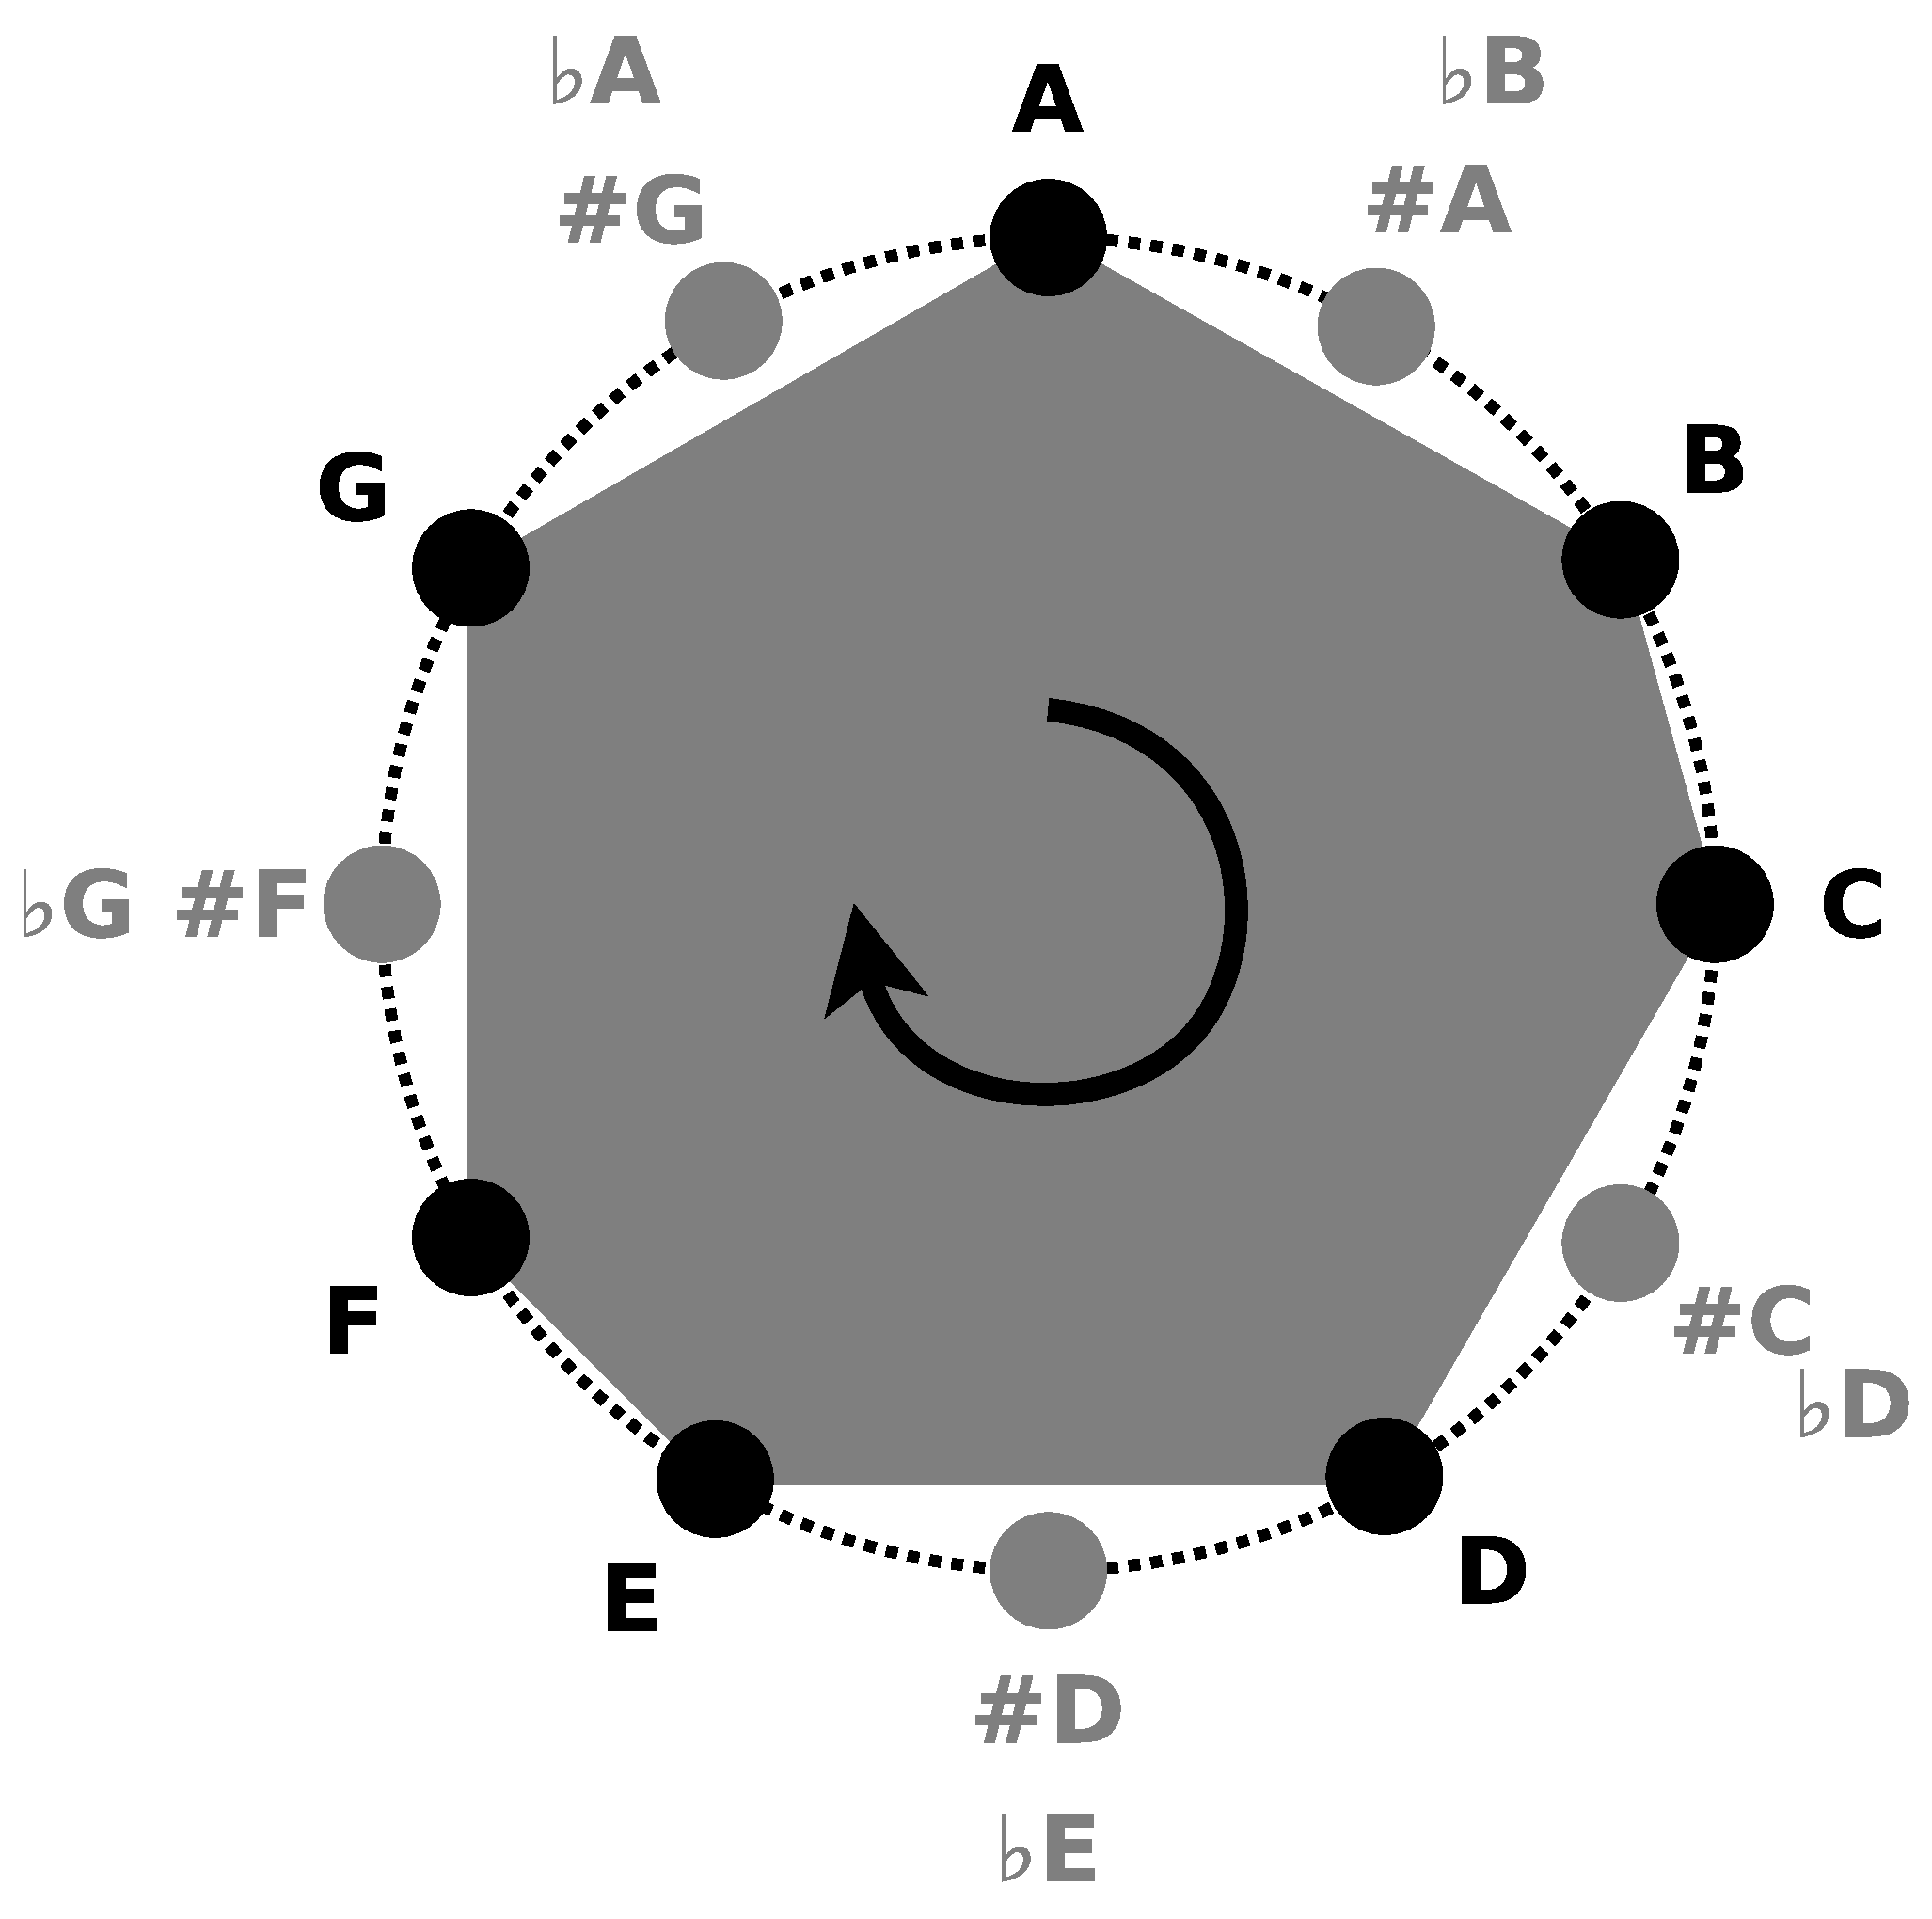
\includegraphics[width=0.65\textwidth]{chapters/cap-musica-basica/circulonotas.eps}
        \caption{Representação cíclica das distancias das notas musicais.}
        \label{fig:circulonotas}
    \end{figure}

Adicionalmente, na Figura \ref{fig:circulonotas}, 
está representada a escala diatônica com uma figura geométrica de 6 lados, 
colorido em cinza; e a escala cromática está representada com um circulo de linha pontuada.




%%%%%%%%%%%%%%%%%%%%%%%%%%%%%%%%%%%%%%%%%%%%%%%%%%%%%%%%%%%%%%%%%%%%%%%%%%%%%%%%
\section{\textcolor{blue}{Tipos de pauta}}
\label{sec:tipospauta}

\subsection{Pauta ou Pentagrama}\index{Pauta}
\label{sec:pauta}
A pauta está representada por 5 linhas paralelas e horizontais, 
as figuras musicais podem ocupar as linhas ou um lugar médio, entre elas.
Adicionalmente lugares fora da pauta podem ser usados; 
para este proposito linhas adicionais e parcialmente desenhadas serão colocadas \cite[pp. 10]{cardoso1973curso},
como é mostrado na Figura \ref{fig:abc-pauta5}.
\begin{figure}[H]
\centering
\begin{abc}[name=abc-pauta5]
% abcm2ps pauta5.abc  -O pauta5.ps
% ps2epsi pauta5.ps pauta5.eps
%
X: 1 % start of header
K: none stafflines=5 %K: C %% Escala de C mayor %
M: none % M: 2/4
%T: Contratempo num compasso binário
V:1 clef=none stem=up name="Pauta"   sname="Pauta"
%
[V:1] C8 D8 E8 F8 G8 A8 B8 C'8 D'8 E'8 F'8 G'8 A'8
\end{abc}
\caption{Pauta com 5 linhas e figuras musicais mostrando algumas posições usáveis.}
\label{fig:abc-pauta5}
\end{figure}
A ordem de leitura das figuras musicais na pauta é de esquerda a direita,
e indica o avanço  do tempo;
as posições das linhas indicam um ordem crescente na altura do som que representam as figuras,
contando desde a linha inferior ate a superior. Nesse sentido, 
uma pauta é semelhante a um espectrograma, onde o eixo X representa o tempo,
o eixo Y representa a frequência, e a figuras colocadas em distintas posições do plano XY, descrevem
o comportamento do sonido nesses dois âmbitos. Assim, a Figura \ref{fig:abc-pauta5}
representa um conjunto de 13 sonidos, cada um com a mesma duração; 
porem, executado com diferentes alturas e em ordem crescente, 
desde um sonido grave ate um sonido mais agudo.


Por outro lado, se as figuras musicais podem ocupar varias posições na partitura,
pois estas representam alturas diferentes  do som,
os silêncios não precisam desta característica,
pelo qual os símbolos que representam os silêncios tem uma posição fixa na pauta,
como pode ser visto na Figura \ref{fig:abc-pautasilencio}.
\begin{figure}[h]
\centering
\begin{abc}[name=abc-pautasilencio]
% abcm2ps pautasilencio.abc  -O pautasilencio.ps
% ps2epsi pautasilencio.ps pautasilencio.eps
%
X: 1 % start of header
K: none stafflines=5 %K: C %% Escala de C mayor %
M: none % M: 2/4
%T: Contratempo num compasso binário
V:1 clef=none name="Pauta"   sname="Pauta"
%
[V:1] z8 z4 z2 z1 z/2 z/4 G8 A4 B2 C'1 D'/2 E'/4 
\end{abc}
\caption{Pauta com 5 linhas e silêncios musicais mostrando algumas posições usáveis.}
\label{fig:abc-pautasilencio}
\end{figure}
O ponto mais interessante, é ver a diferencia do uso  da pausa de mínima e a pausa de semibreve,
dado que estes dois tipos de pausa usam o mesmo simbolo, porem em distintas posições.
Na Figura \ref{fig:abc-pautasilencio} a pausa de semibreve, 
está colocada em primeiro lugar desde a esquerda da pauta,
e o simbolo está desenhado unido a parte baixa da quarta linha da pauta, contando desde abaixo.
Por outro lado, a pausa de mínima está desenhada no segundo lugar da pauta,
contando desde a esquerda, e se desenha unida parte de acima da 3 linha da pauta.

\subsubsection{As claves na pauta}
Existem 3 tipos de claves\footnote{E varias posições para estas} que podem ser usadas na pauta, 
assim temos: 
\begin{itemize}
\item clave sol, 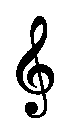
\includegraphics[height=14pt]{chapters/cap-musica-basica/G-clef.eps},
\item a clave de fá, 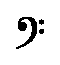
\includegraphics[height=10pt]{chapters/cap-musica-basica/FClef.eps}, e 
\item a clave de dó, 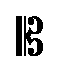
\includegraphics[height=10pt]{chapters/cap-musica-basica/CClef.eps}.
\end{itemize}
A clave, como símbolo, se coloca ao inicio da pauta, e serve para indicar as alturas das notas na pauta \cite[pp. 179]{apel1969harvard} \cite[pp. 10]{cardoso1973curso}.

Figura \ref{fig:allclaves}
\begin{figure}[h]
    \centering
\begin{subfigure}[b]{\textwidth}
\caption{Clave de sol.}
\begin{abc}[name=abc-clavesol]
% abcm2ps clavesol.abc  -O clavesol.ps
% ps2epsi clavesol.ps clavesol.eps
%
X: 1 % start of header
K: C stafflines=5 %K: C %% Escala de C mayor %
M: none % M: 2/4
%T: Contratempo num compasso binário
V:1 clef=treble %name="Pauta com clave de sol"   sname="Pauta com clave de sol"
%
[V:1] "dó"C,8 "ré"D,8 "mi"E,8 "fá"F,8  "sol"G,8 "lá"A,8 "si"B,8 "dó"C8 "ré"D8 "mi"E8 "fá"F8  "sol"G8 "lá"A8 "si"B8 "dó"C'8 
\end{abc}
\label{fig:abc-clavesol}
\end{subfigure}
~ %
\begin{subfigure}[b]{\textwidth}
\caption{Clave de fá.}
\begin{abc}[name=abc-clavefa]
% abcm2ps clavesfa.abc  -O clavefa.ps
% ps2epsi clavefa.ps clavefa.eps
%
X: 1 % start of header
K: C stafflines=5 %K: C %% Escala de C mayor %
M: none % M: 2/4
%T: Contratempo num compasso binário
V:1 clef=bass %name="Pauta com clave de fá"   sname="Pauta com clave de fá"
%
[V:1] "dó"C,8 "ré"D,8 "mi"E,8 "fá"F,8  "sol"G,8 "lá"A,8 "si"B,8 "dó"C8 "ré"D8 "mi"E8 "fá"F8  "sol"G8 "lá"A8 "si"B8 "dó"C'8 
\end{abc}
\label{fig:abc-clavefa}
\end{subfigure}
~ %
\begin{subfigure}[b]{\textwidth}
\caption{Clave de dó.}
\begin{abc}[name=abc-clavedo]
% abcm2ps clavesfa.abc  -O clavedo.ps
% ps2epsi clavedo.ps clavedo.eps
%
X: 1 % start of header
K: C stafflines=5 %K: C %% Escala de C mayor %
M: none % M: 2/4
%T: Contratempo num compasso binário
V:1 clef=C %name="Pauta com clave de fá"   sname="Pauta com clave de fá"
%
[V:1] "dó"C,8 "ré"D,8 "mi"E,8 "fá"F,8  "sol"G,8 "lá"A,8 "si"B,8 "dó"C8 "ré"D8 "mi"E8 "fá"F8  "sol"G8 "lá"A8 "si"B8 "dó"C'8 
\end{abc}
\label{fig:abc-clavedo}
\end{subfigure}
    \caption{Tipos de claves}\label{fig:allclaves}
\end{figure}

\subsection{\textcolor{red}{Pauta de percussão}}\index{Pauta!Pauta de Percussão}

\subsubsection{The monolinear system of notation}
notation created by Dr. Fritz Berger of Basel, Switzerland that he called The Monolinear System of Notation

Figura \ref{fig:abc-monolinearperc}
\begin{figure}[H]
\centering
\begin{abc}[name=abc-monolinearperc]
% abcm2ps monolinearperc.abc  -O monolinearperc.ps
% ps2epsi monolinearperc.ps monolinearperc.eps
%
X: 1 % start of header
K: none stafflines=1 %K: C %% Escala de C mayor %
M: none % M: 2/4
%T: Contratempo num compasso binário
V:1 clef=perc stem=up name="Ritmo 1"   sname="Ritmo 1"
%
[V:1] "S/4"B2 "S/16"B/2 "S/8"B1 "S/8"B1 "S"B8  "S/2"B4  |

\end{abc}
\caption{Figuras e pausas}
\label{fig:abc-monolinearperc}
\end{figure}


\subsubsection{The musical notation of percusion}
Figura \ref{fig:abc-musicalperc}
\begin{figure}[H]
\centering
\begin{abc}[name=abc-musicalperc]
% abcm2ps musicalperc.abc  -O musicalperc.ps
% ps2epsi musicalperc.ps musicalperc.eps
%
X:1
T:Drum Key
M:
L:1/4
K:C clef=perc
"^Bass"F|"^Snare"c|"^High tom"e|"^Mid tom"d|"^Low tom"B|"^Floor tom"A|
"^Cymbal"^b|"^Crash"^a|"^Hi-hat"^g|"^Ride"^f|"^Hi-hat Pedal"^D|]

\end{abc}
\caption{Figuras e pausas}
\label{fig:abc-musicalperc}
\end{figure}

\subsubsection{The grid notation}

%%%%%%%%%%%%%%%%%%%%%%%%%%%%%%%%%%%%%%%%%%%%%%%%%%%%%%%%%%%%%%%%%%%%%%%%%%%%%%%%
\section{\textcolor{green}{Compasso}}\index{Compasso}
\label{sec:compaso}

\begin{description}
\item[Compasso:] O dicionário de Harvard de música \cite[pp. 513]{apel1969harvard} define compasso (``measure'' em inglês)
como um grupo de tempos, batimentos ou pulsos (unidade do tempo musical),
onde o primeiro destes normalmente é acentuado. 
Este número de tempos no compasso pode ser, dois, trés, quatro, ou ocasionalmente 5 ou mais. 
Sendo estos compassos separados por barras verticais e as notas do compasso esquematizados baixo uma métrica.
\begin{example}
Figura \ref{fig:abc-exemplocompasso1}
\end{example}
 
\item[Métrica:] Sobre a métrica  (``meter'' em inglês) o dicionario \cite[pp. 523]{apel1969harvard} explica que é
um padrão de unidades temporais fixas, chamados batimentos, 
pelo qual um período de tempo de uma peça musical ou uma seção dela é medida. 
Agrega tambem que a métrica é indicado geralmente por uma fração, como por exemplo:
${2}/{2}$ , ${3}/{4}$ , ${4}/{4}$, etc. Em português esta fração é chamada de formula do compasso. 
\begin{example}
Figura \ref{fig:abc-exemplocompasso1}
\end{example}
\end{description}

O numerador, da formula do compasso, indica o número de pulsações (tempos) que compõem cada compasso.
Por outro lado o denominador nos informa al longitude temporal de cada um dos tempos do compasso.

\begin{figure}[h]
\centering
\begin{abc}[name=abc-exemplocompasso1]
% abcm2ps exemplocompasso1.abc  -O exemplocompasso1.ps
% ps2epsi exemplocompasso1.ps exemplocompasso1.eps
%
X: 1 % start of header
K: none stafflines=0 %K: C %% Escala de C mayor %
M: 2/4
%T: Contratempo num compasso binário
V:1 clef=perc stem=up name="Ritmo 1"   sname="Ritmo 1"
%
[V:1] | B2 B1 B1| B2 B1 B1 | B2 B1 B1 | B2 z2  |
%       
\end{abc}
\caption{Figuras e pausas}
\label{fig:abc-exemplocompasso1}
\end{figure}



A Tabela \ref{tab:abc-noteslength} exemplifica o significado do denominador da formula do compasso; 
\begin{table}[h]
\centering
\begin{tabular}{|c|c|c|c|}
\hline
denominador & Figura  & Duração & Nome\\ \hline
\hline
$1$   & \fullnote    & $S$   & Semibreve \\ \hline
$2$ & \halfnote    & $S/2$ & Mínima \\ \hline
$4$ & \quarternote & $S/4$ & Semínima \\ \hline
$8$ & \eighthnote  & $S/8$ & Colcheia \\ \hline
\end{tabular}
\caption{Duração e símbolos de algumas figuras musicais}
\label{tab:abc-noteslength}
\end{table}
onde a primeira coluna mostra o denominador da formula,
a segunda coluna mostra as figuras musicais que representam cada um dos tempos do compasso, e 
a terceira e quarta coluna, indicam a duração em segundos e o nome da figura musical.

podemos achar equivalências aos exemplos da formula do compasso dados
anteriormente; onde os compassos com formula $\mathbf{2}/2$ tem cada um, uma duração de $\mathbf{2}$\halfnote ~(duas mínimas),  
compassos com formula $\mathbf{3}/4$ tem uma duração de $\mathbf{3}$\quarternote ~(trés semínimas) 
e $\mathbf{4}/4$ uma duração de $\mathbf{4}$\quarternote ~(quatro semínimas). É importante
ressaltar que a duração em tempo das figuras musicais é relativa, como pode ser visto
na terceira coluna da Tabela \ref{tab:abc-noteslength}, onde as durações estão em função
da duração $S$ da semibreve. 


Se classificamos os compassos por sua métrica, os três tipos mais conhecidos 
são os compassos binários, ternários, quaternários \cite[pp. 27]{adolfo2002musica}.

\subsection{\textcolor{green}{Compasso binário}}\index{Compasso!Compasso Binário} Ou compasso binário simples,
é uma estrutura rítmica que se carateriza por ter compassos com uma  duração de dois tempos,
sendo o primeiro tempo forte (acentuado), e o segundo de tempo fraco (não acentuado)
\cite[pp. 41]{grabner2001teoria} \cite[pp. 66]{adolfo2002musica}\cite[pp. 28]{alves2004teoria}. 
Os compassos binários (simples) tem uma formula de compasso na forma $2/B$,
onde $B$ pode ser $2$, $4$, $8$, etc. 
A Figura \ref{compasso:binario}, representa um exemplo de compasso binário simples, 
com formula de compasso $2/2 \equiv 2$\halfnote, 
e tempos com uma duração de $S/2$ (uma \halfnote), 
sendo que o primeiro compasso contem $2$\halfnote~e o segundo contem $4$\quarternote.
Na Figura \ref{compasso:binario} a sigla ``N.A.'' significa ``Não acentuado'', pelo que é fácil perceber
que em qualquer caso, só a nota que é executada no tempo 1 é acentuada.
\begin{figure}[H]
\centering
\begin{abc}[name=abc-compasso1]
X: 1 % start of header
K: C % scale: C major
M: 2/2 %meter - compasso
"Primeiro compasso" G4 F4 |"Segundo compasso" G2 D2 F2 D2  |
w: Acentuado N.A. Acentuado N.A. N.A. N.A.
\end{abc}
\caption{Exemplo de compasso binário (simples)}
\label{compasso:binario}
\end{figure}

Se falamos de forma mais geral, 
podemos ter dois tipos de compassos binários: os simples e os compostos.
Assim, 
para achar a formula de um compasso composto, correspondente a um compasso simples (usando quialteras de três)
usamos a seguinte operação \cite[pp. 74]{alves2004teoria}, 
\begin{equation}\label{eq:comcomposto}
Compasso~simples\times\frac{3}{2}=Compasso~composto.
\end{equation}
De modo que obtemos compassos binários compostos com as seguintes formulas de compasso: 
$6/4$, $6/8$, $6/16$, etc.
A diferencia do visto nos compassos binários simples, os compassos binários compostos tem 
um pulso forte (Acentuado) no tempo 1 e um pulso semiforte (Acentuado porem menor) no tempo 4, 
de modo que os tempos 2,3,5 e 6,
são classificados como tempos fracos (Não Acentuados)\cite[pp. 41]{grabner2001teoria}.
A Figura \ref{compasso:binariocomposto}, representa um exemplo de compasso binário composto, 
com formula de compasso $6/4 \equiv 6$\quarternote, 
e tempos com uma duração de $S/4$ (uma \quarternote), 
sendo que o primeiro compasso contem $6$\quarternote~e o segundo contem dois $2$\quarternote~e dois $2$\halfnote.
Da Figura \ref{compasso:binariocomposto} é fácil perceber
que em qualquer caso, só são acentuados as nota que são executadas no tempo 1 e 4; 
aclarando que as notas executadas no tempo 4 tem uma acentuação menor que as executadas no tempo 1.
\begin{figure}[H]
\centering
\begin{abc}[name=abc-compasso1c]
X: 1 % start of header
K: C % scale: C major
M: 6/4 %meter - compasso
"Primeiro compasso" G2 D2 D2 F2 D2 D2 |"Segundo compasso" G2 D4 F2 D4  |
w: Acentuado N.A. N.A. Acentuado N.A N.A. Acentuado N.A. Acentuado N.A. 
\end{abc}
\caption{Exemplo de compasso binário composto}
\label{compasso:binariocomposto}
\end{figure}

Alguns autores consideram aos compassos quaternários (ex: 4/4, 4/8) como um caso de compasso binário,
chamando eles de compasso binário duplo \cite[pp. 41]{grabner2001teoria}.




\subsection{\textcolor{green}{Compasso ternário}}\index{Compasso!Compasso Ternário} Ou compasso ternário simples,
é uma estrutura rítmica que se carateriza por ter compassos com trés tempos,
sendo o primeiro pulso forte (acentuado) e os outros dois fracos (não acentuados) 
\cite[pp. 67]{adolfo2002musica}\cite[pp. 30]{alves2004teoria}. 
Os compassos ternários (simples) tem uma formula de compasso da forma $3/B$, 
onde $B$ pode ser $2$, $4$, $8$, etc.
Por exemplo temos, as formulas de compassos ternários simples: $3/2$, $3/4$, $3/8$,  etc.

A Figura \ref{compasso:ternario}, representa um exemplo de compasso ternário (simples), com 
formula de compasso $3/4 \equiv 3$\quarternote, 
onde os tempos tem uma duração de $S/4$, o primeiro compasso contem $3$\quarternote~e
o segundo contem $6$\eighthnote.
Na Figura \ref{compasso:ternario}  é fácil perceber
que em ambos compassos, só a nota que é executada no tempo 1 é acentuada.
\begin{figure}[H]
\centering
\begin{abc}[name=abc-compasso2]
X: 1 % start of header
K: C % scale: C major
M: 3/4 %meter - compasso
"Primeiro compasso" G2 F2 F2 |"Segundo compasso" G1 F1 E1 D1 D1  D1  |
w: Acentuado N.A. N.A. Acentuado N.A N.A.  N.A. N.A. N.A. 
\end{abc}
\caption{Exemplo de compasso ternário}
\label{compasso:ternario}
\end{figure}


São chamados de compassos ternários compostos,  
quando estes tem uma formula de compasso como: $9/4$, $9/8$ e $9/16$.
Para gerar estes compassos compostos a partir de suas versões simples,
se segue a mesma operação descrita na Equação \ref{eq:comcomposto}.


\subsection{\textcolor{green}{Compasso quaternário}}\index{Compasso!Compasso Quaternário} Ou compasso quaternário simples,
é uma estrutura rítmica que se carateriza por ter compassos com quatro tempos,
sendo o primeiro pulso forte (acentuado), o segundo fraco (não acentuado), 
o terceiro semiforte (acentuado porem menor) e o último fraco (não acentuado) 
\cite[pp. 67]{adolfo2002musica}\cite[pp. 32]{alves2004teoria}. 
Os compassos quaternários (simples) tem uma formula de compasso da forma $4/B$, 
onde $B$ pode ser $2$, $4$, $8$, etc.
Por exemplo temos, as formulas de compassos ternários simples: $4/2$, $4/4$, $4/8$,  etc.

A Figura \ref{compasso:quaternario}, representa um exemplo de compassos quaternário, com 
formula de compasso $4/4 \equiv 4$\quarternote, 
onde cada tempo tem uma duração de $S/4$, o primeiro compasso contem $4$\quarternote~e
o segundo contem $8$\eighthnote.
Na Figura \ref{compasso:ternario}  é fácil perceber
que em ambos compassos, só as notas que são executadas no tempo 1 e 3 são acentuadas.
\begin{figure}[H]
\centering
\begin{abc}[name=abc-compasso3]
X: 1 % start of header
K: C % scale: C major
M: 4/4 %meter - compasso
"Primeiro compasso" G2 D2 F2 D2|"Segundo compasso" G1 F1 D1 C1 F1 E1 D1 C1 |
w: Acentuado N.A. Acentuado N.A. Acentuado N.A N.A. N.A. Acentuado N.A. N.A. N.A. 
\end{abc}
\caption{Exemplo de compasso quaternário}
\label{compasso:quaternario}
\end{figure}

São chamados de compassos quaternários compostos,  
quando estes tem uma formula de compasso como: $12/4$, $12/8$ e $12/16$.
Para gerar estes compassos compostos a partir de suas versões simples,
se segue a mesma operação descrita na Equação \ref{eq:comcomposto}.
 


%%%%%%%%%%%%%%%%%%%%%%%%%%%%%%%%%%%%%%%%%%%%%%%%%%%%%%%%%%%%%%%%%%%%%%%%%%%%%%%%
\section{\textcolor{blue}{Tempo}}\index{Tempo}

Como já foi sugerido na Seção \ref{sec:compaso}, é chamado de "tempo" 
à pulsação básica e unidade de medida dos compassos nas composições musicais;
assim, temos que compassos binários, ternários e quaternários; que tem uma duração de 2 tempos, 
3 tempos e 4 tempos, respetivamente. Por comodidade designaremos com a variável $T$ à duração em segundos de cada tempo,
sendo que o valor de $T$ variará dependendo da formula de compasso usada.

\subsection{\textcolor{red}{Tempo forte}}\index{Tempo!Tempo Forte}


\subsection{\textcolor{red}{Tempo fraco}}\index{Tempo!Tempo Fraco}

\subsection{\textcolor{green}{O tempo em diferentes formula de compasso}}
É importante ressaltar que os compassos que usem a mesma formula de compasso terão sempre a mesma duração em segundos;
por outro lado, podem ser achados casos onde compassos com diferente formula podem ter a mesma duração;
por exemplo: compassos binários com formula $\mathbf{2}/2$, comparados com compassos quaternários com 
formula $\mathbf{4}/4$; ambos compassos tem a mesma duração uma semibreve (\fullnote).

Na Figura \ref{fig:abc-tempo1} podemos ver compassos binários com formula $\mathbf{2}/2$, 
\begin{figure}[H]
\centering
\begin{abc}[name=abc-tempo1]
X: 1 % start of header
K: C % scale: C major
M: 2/2 %meter - compasso
G2 D2 F2 D2 | G4 F4 |
w: T/2 T/2 T/2 T/2  T T
\end{abc}
\caption{Exemplo de dois compassos com 2 tempos de duração T}
\label{fig:abc-tempo1}
\end{figure}
onde estos terão uma duração de dois tempos ($2T$) \cite[pp. 25]{azevedocompor} onde cada tempo ($T$) tem uma duração 
de uma mínima (\halfnote), ver Tabela \ref{tab:abc-noteslength};
por outro lado,
compassos quaternários com formula $\mathbf{4}/4$, como na Figura \ref{fig:abc-tempo2}, 
\begin{figure}[H]
\centering
\begin{abc}[name=abc-tempo2]
X: 1 % start of header
K: C % scale: C major
M: 4/4 %meter - compasso
G2 D2 F2 D2| G4 F4|
w: T T T T 2T 2T
\end{abc}
\caption{Exemplo de dois compassos com 4 tempos de duração T}
\label{fig:abc-tempo2}
\end{figure} 
terão uma duração de 4 tempos ($4T$) \cite[pp. 25]{azevedocompor} onde 
cada tempo ($T$) tem uma duração de uma semínima (\quarternote), ver Tabela \ref{tab:abc-noteslength}.
Assim, estas duas formulas ($2/2$ e $4/4$) representam compassos 
com a mesma duração em segundos, uma semibreve (\fullnote),
porem tem valores diferentes para a variável $T$ em segundos.

\begin{lattention}
Se interpretamos a música mostrada nas Figuras \ref{fig:abc-tempo1} e \ref{fig:abc-tempo2},
podemos perceber que ambas descrevem um sonido ligeiramente diferente; assim, não é fácil
distinguir se o sonido provem de um compasso com formula $2/2$ ou $4/4$.
Em estes casos a dica é perceber se existem dois tipos de tempos fortes, acentuados
com diferentes intensidades; se é assim, então estamos ante um compasso quaternário;
se não, então é um compasso binário.
\end{lattention}


\subsection{\textcolor{red}{Contagem dos tempos no compasso}}


%%%%%%%%%%%%%%%%%%%%%%%%%%%%%%%%%%%%%%%%%%%%%%%%%%%%%%%%%%%%%%%%%%%%%%%%%%%%%%%%
\section{\textcolor{green}{Contratempo}}\index{Contratempo}
Um contratempo acontece quando as notas (representadas por figuras musicais na partitura) 
são executadas em tempos fracos do compasso
ou nas partes fracas dos tempos, sendo que estas estão intercaladas por pausas nos tempos
fortes ou partes fortes dos tempos \cite[pp. 16]{mascarenhascurso} 
\cite[pp. 36]{azevedocompor}, neste sentido o contratempo pode ser visto como a 
omissão de notas nos tempos fortes ou nas partes fortes dos tempos \cite[pp. 146]{medteoria}.
Ou ``num sentido mais amplo, o contratempo é a acentuação de um tempo fraco em vez de um tempo forte'' \cite[pp. 147]{medteoria}. 

Assim, a palavra ``contratempo'', referencia a como estão configuradas ou acentuadas 
as notas no compasso. Por exemplo:
A Figura \ref{fig:contratempoa} mostra 
quatro compassos (binários) com formula $2/4$, em cada compasso existem 
contratempos nos tempos fracos ou nas partes fracas dos tempos, sendo que cada tempo
tem uma duração de uma semínima (\quarternote) e cada compasso uma duração 
de uma mínima (\halfnote), ou seja duas semínimas (2\quarternote). 
\begin{itemize}
\item ``F''  indica que é o tempo é forte, 
\item ``f''  indica que é o tempo é fraco,
\item ``FF'' indica que é a parte forte de um tempo forte,
\item ``Ff'' indica que é a parte fraca de um tempo forte,
\item ``fF'' indica que é a parte forte de um tempo fraco,
\item ``ff'' indica que é a parte fraca de um tempo fraco, 
\end{itemize} 

finalmente
a figura musical \ViPa~ indica um silencio da mesma duração que uma semínima (\quarternote)
e a figura musical \AcPa~ indica um silencio da mesma duração que uma colcheia (\eighthnote).
\begin{figure}[H]
\centering
\begin{abc}[name=abc-contratempoa]
X: 1 % start of header
K: C % scale: C major
M:2/4
%T: Contratempo num compasso binário
V:1 clef=treble name="A" sname="A"
[V:1] "F"z2 "f"G2 | "FF"z1 "Ff"G1  "fF"z1 "ff"G1 | "FF"z1 "Ff"G1  "f"G2 |  "F"z2 "fF"z1 "ff"G1  |
w:          T          T/2            T/2             T/2     Tempo                 T/2
\end{abc}
\caption{Contratempos no tempos fracos ou nas partes fracas dos tempos}
\label{fig:abc-contratempoa}
\end{figure}
Na Figura \ref{fig:abc-contratempoa}, existem contratempos em todos os compassos porem estes estão
configurados de distintas formas;
no primeiro compasso acontece um contratempo dado que a única nota é executada 
no tempo fraco do compasso, no segundo compasso acontecem contratempos pois as 
notas são executadas nas partes fracas de cada tempo,
no terceiro compasso acontece um contratempo pela execução de uma nota na parte 
fraca do tempo forte, sendo o resto do tempo preenchido com um silencio, e 
finalmente no quarto compasso acontece um contratempo pela execução de uma nota
na parte fraca do tempo fraco, sendo o resto do compasso preenchido com silêncios.


Por outro lado, 
a Figura \ref{fig:abc-contratempob} mostra um caso similar ao da Figura \ref{fig:abc-contratempoa},
com contratempos expressados como a acentuação de um tempo fraco em vez de um silencio no tempo forte \cite[pp. 147]{medteoria}. 
É usado o símbolo $>$ para indicar esta acentuação na partitura.
\begin{figure}[H]
\centering
\begin{abc}[name=abc-contratempob]
X: 1 % start of header
K: C % scale: C major
M:2/4
%T: Contratempo num compasso binário
V:1 clef=treble name="A" sname="A"
[V:1] "F"G2 "f"+accent+G2 | "FF"G1 "Ff"+accent+G1  "fF"G1 "ff"+accent+G1 | "FF"G1 "Ff"+accent+G1  "f"G2  | "F"G2 "fF"G1  "ff"+accent+G1  | 
w:    T     T                T/2    T/2             T/2    T/2              T/2    T/2             T       T      T/2             T/2  
\end{abc}
\caption{Contratempos pela acentuação dos tempos fracos ou nas partes fracas dos tempos}
\label{fig:abc-contratempob}
\end{figure}

%%%%%%%%%%%%%%%%%%%%%%%%%%%%%%%%%%%%%%%%%%%%%%%%%%%%%%%%%%%%%%%%%%%%%%%%%%%%%%%%
\section{\textcolor{red}{Sincopa}}\index{Sincopa}




